\documentclass[]{article}
\usepackage[numbers]{natbib}
\usepackage{amsfonts, amssymb, amsmath}
\usepackage{url}
\usepackage{float}
\usepackage{graphicx}
\usepackage{adjustbox}
\usepackage[colorlinks=true, allcolors=blue]{hyperref}
\usepackage[]{geometry}
\usepackage{url}
\usepackage{tikz, pgfplots}
\usepackage{multicol}
\usetikzlibrary{positioning, shapes.geometric, arrows}

\title{Proposed Skew Model}
\author{
  Thomas, Harper\\
  \texttt{zeroknowledgeltd@gmail.com}
}

\date{\today}

\begin{document}

\maketitle

\section{SNX v3 Skew Funding Rate}

The skew funding rate is used to protect LPs against directional risk. It is a function of the market funding velocity over time. Funding velocity is determined by market skew, which is the sum of all traders positions in the market.

\begin{equation}
K := \sum_{c \in C}{q^c} = Q_L - Q_S
\end{equation}

The skew funding rate is paid by traders to other traders, and is used to incentivise traders (or arbitrageurs) to take the other side of the market when it is skewed. Funding velocity as a price discovery mechanism, that allows the funding rate to drift upwards or downwards on a daily basis to find a level at which market participants are sufficiently motivated to take action and balance skew by taking the other side of the market.\\

The market administrator manages the intensity of skew funding by setting the max skew funding velocity $I^s_{max}$ and the $skewScale$ parameter.

\begin{equation}
W := \frac{K}{skewScale} = \textit{Proportional Skew}
\end{equation}
\begin{equation}
W_{\textit{bounded}} = clamp(W, -1, 1)
\end{equation}
\begin{equation}
I^s = W_{\textit{bounded}}\cdot I^s_{max} = Skew Funding Velocity
\end{equation}

The skew scale, determines the level of skew at which the maximum funding velocity will be achieved.

\subsection{SNX V3 Funding Velocity}

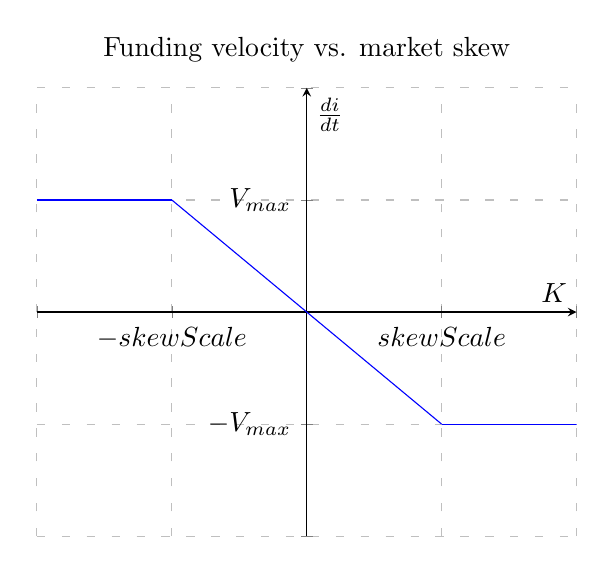
\begin{tikzpicture}
\begin{axis}[
    title={Funding velocity vs. market skew},
    xmin=-2, xmax=2,
    ymin=-2, ymax=2,
    axis lines=middle,
    xlabel=$K$,
    ylabel=$\frac{di}{dt}$,
    xtick={-2, -1, 0, 1, 2},
    xticklabels={, $-skewScale$, , $skewScale$},
    ytick={-2, -1, 0, 1, 2},
    yticklabels={, $-V_{max}$, , $V_{max}$, ,},
    ymajorgrids=true,
    xmajorgrids=true,
    grid style=loosely dashed,
]
\addplot[color=blue, samples=100, domain=-1:1]{-x};
\addplot[color=blue, samples=100, domain=1:2]{-1};
\addplot[color=blue, samples=100, domain=-2:-1]{1};
\end{axis}
\end{tikzpicture}

\subsection{SNX V3 Funding Acceleration}

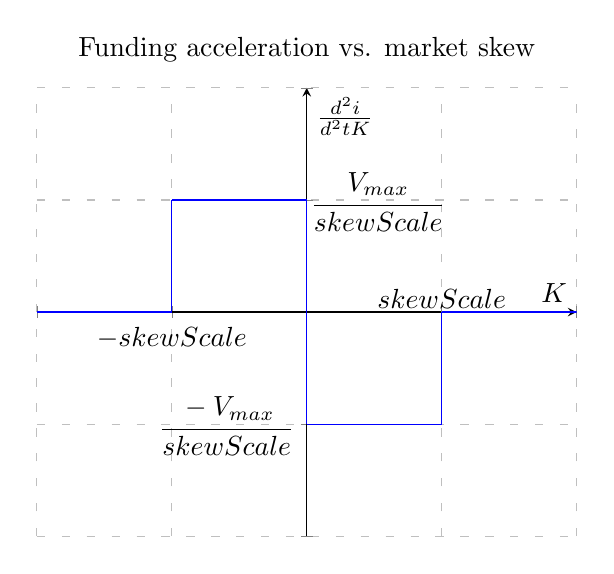
\begin{tikzpicture}
\begin{axis}[
    title={Funding acceleration vs. market skew},
    xmin=-2, xmax=2,
    ymin=-2, ymax=2,
    axis lines=middle,
    xlabel=$K$,
    xtick={-2, -1},
    xticklabels={, $-skewScale$},
    extra x ticks={1, 2},
    extra x tick labels={$skewScale$,},
    extra x tick style={
        xticklabel style={anchor=south}
    },
    xticklabel style={anchor=north},
    ylabel=$\frac{d^2i}{d^2tK}$,
    ytick={-2, -1},
    yticklabels={, $\cfrac{-V_{max}}{skewScale}$},
    yticklabel style={anchor=east},
    extra y ticks={1, 2},
    extra y tick labels={$\cfrac{V_{max}}{skewScale}$,},
    extra y tick style={
        yticklabel style={anchor=west}
    },
    ymajorgrids=true,
    xmajorgrids=true,
    grid style=loosely dashed,
]
\addplot[color=blue, samples=100, domain=-2:-1]{0};
\addplot[color=blue] coordinates {(-1, 0) (-1, 1)};
\addplot[color=blue, samples=100, domain=-1:0]{1};
\addplot[color=blue] coordinates {(0, 1) (0, -1)};
\addplot[color=blue, samples=100, domain=0:1]{-1};
\addplot[color=blue] coordinates {(1, -1) (1, 0)};
\addplot[color=blue, samples=100, domain=1:2]{0};
\end{axis}
\end{tikzpicture}


\section{Proposed Skew Funding Rate}

I propose a slightly different model which removes the need for $skewScale$ and allows the market to dynamically respond to changing market conditions and available liquidity.\\



\end{document}
